
\documentclass{article}
\usepackage{graphicx}
\usepackage{geometry}
\usepackage{multicol}


% Ajustar los márgenes para que todo quepa en una página
\geometry{
    a4paper,
    total={170mm,257mm},
    left=20mm,
    top=10mm,
}

\begin{document}


\begin{flushright} % Alinea el logo a la derecha
    
\includegraphics[width=1.5cm]{tex/media/logo.png} 
\end{flushright}

\centering
{\Huge \textbf{Informe}}

\vspace{0.5cm}

{\Large Autogenerado por XaiCreditCopilot}

\vspace{0.5cm}

{\large \today}

\raggedright

El presente informe ha sido autogenerado con el propósito de cumplir con el plan de seguimiento posterior del proyecto. Toda la información contenida en este documento se proporciona únicamente como un hecho informativo para evaluar el funcionamiento adecuado del sistema.

\begin{multicols}{2}

En el presente documento se muestran estadísticas creadas por el sistema durante el último mes. Podemos apreciar cómo se han realizado {\huge 27 inferencias} con el sistema y se han generado conclusiones relevantes sobre el proceso de otorgamiento de créditos. Los siguientes gráficos representan la distribución de la aceptación y denegación de crédito en función de variables protegidas, como género, nacionalidad, tipo de trabajo y estado civil. Estos análisis son cruciales para identificar posibles sesgos en el proceso de toma de decisiones y garantizar la equidad en el acceso al crédito.

\vspace{0.5cm}
\textbf{Análisis por género:}

En primer lugar, podemos apreciar dos gráficos de tarta que representan la distribución de créditos aceptados y denegados según el género de los solicitantes. Estos gráficos proporcionan una visión clara de la proporción de créditos otorgados y rechazados para mujeres y hombres. Además, se muestra el total de créditos solicitados por cada género, lo que permite una comparación directa entre la cantidad de créditos solicitados por mujeres y hombres.

\begin{center} % Alinea el logo a la derecha
    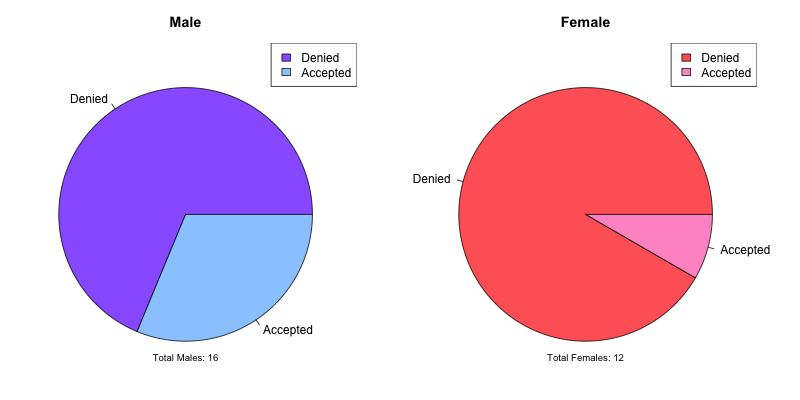
\includegraphics[width=8cm]{tex/media/gender.png} 
\end{center}

Después de un análisis exhaustivo de los registros, la aplicación ha concluido que es pertinente {\huge otorgar un 22\%} de los créditos evaluados durante este período.

\vspace{0.5cm}
\textbf{Análisis por extranjería:}

Uno de los aspectos clave que se analizan en este estudio es el estatus de extranjería del solicitante. Este factor desempeña un papel fundamental en el proceso de evaluación de créditos, ya que puede influir en la decisión final sobre la aprobación o denegación del crédito. A continuación, se presentan los hallazgos relacionados con la distribución de créditos en función del estatus de extranjería de los solicitantes.


\begin{center} % Alinea el logo a la derecha
    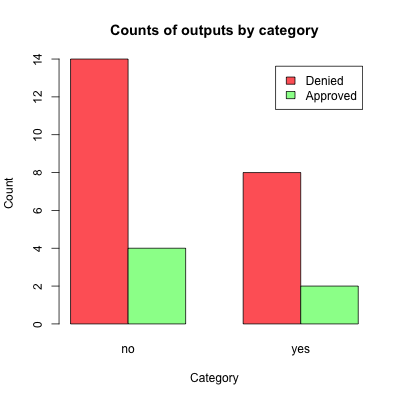
\includegraphics[width=8cm]{tex/media/foreign.png} 
\end{center}

\vspace{0.5cm}
\textbf{Análisis por tipo de empleo:}

Otro aspecto relevante que se considera en este análisis es el puesto de trabajo del solicitante. Este factor se examina con detenimiento para evitar sesgos por nivel educativo en el conjunto de datos. Dado que el tipo de trabajo puede estar correlacionado con el nivel de ingresos y estabilidad laboral, comprender su distribución en relación con la aprobación o denegación de créditos es esencial para garantizar la equidad en el proceso de evaluación. A continuación, se presentan los resultados relacionados con la distribución de créditos según el puesto de trabajo de los solicitantes.


\begin{center} % Alinea el logo a la derecha
    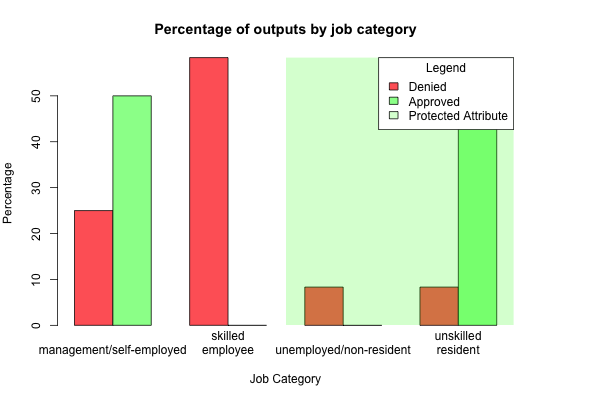
\includegraphics[width=8cm]{tex/media/jobs.png} 
\end{center}

\vspace{0.5cm}
\textbf{Análisis por estadi civil:}

Otro aspecto relevante bajo estudio es el estado civil del solicitante. Reconociendo que el estado civil, como estar casado, puede conferir ciertos privilegios en algunas circunstancias, es esencial examinar su impacto en el proceso de evaluación de créditos. 

\begin{center} % Alinea el logo a la derecha
    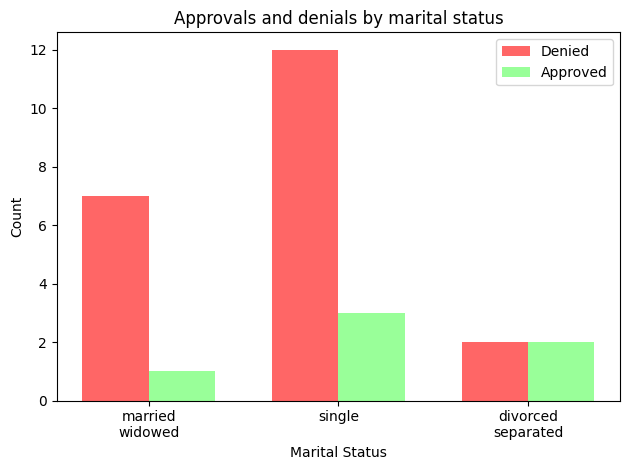
\includegraphics[width=8cm]{tex/media/marital.png} 
\end{center}

Es fundamental comprender cómo se distribuyen los créditos según diversos atributos protegidos de los solicitantes para identificar posibles sesgos y garantizar la imparcialidad en el proceso de otorgamiento.

\end{multicols}

A continuación, se presenta una gráfica que ilustra la evolución temporal de las inferencias, reflejando la cantidad de créditos otorgados en distintos períodos.

\begin{center} % Alinea el logo a la derecha
    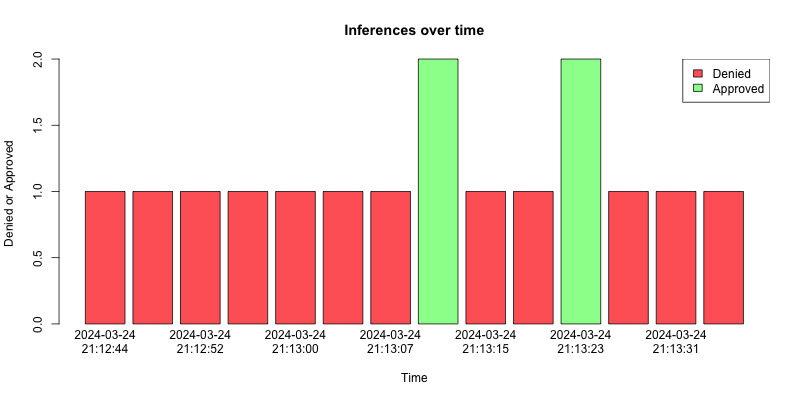
\includegraphics[width=16cm]{tex/media/sequence.png} 
\end{center}

En conclusión, revisar periódicamente el informe es crucial para asegurar que el modelo de inferencia opere de manera adecuada y sin sesgos en relación a los distintos atributos a lo largo del tiempo. Esta práctica no solo garantiza la precisión y fiabilidad de las decisiones tomadas por el sistema, sino que también promueve la equidad y transparencia en el proceso de evaluación de créditos.


Con aprecio y dedicación,

XaiCreditCopilot

\begin{center}
    \textbf{Con aprecio y dedicación,}\\
    \vspace{0.5cm}
    \textsc{XaiCreditCopilot}\\
    \vspace{0.2cm}
\end{center}

{\small
Gracias por confiar en nuestro sistema para el análisis y evaluación de créditos. Estamos comprometidos a seguir mejorando y garantizar la equidad y precisión en cada decisión. No dudes en contactarnos si alguno de los parámetros difiere de un rango normal.
}

\end{document}

